% =====================================================================
%  EnergyMind Tunisia -- Human-AI Escalation and Governance (Challenge Goal 3).
%  LaTeX rebuild of human_ai_escalation_governance_report.pdf (originally printed
%  from HTML), with the fixes from the N1 dataset-compatibility review applied:
%  asset-criticality overlay, severity from scope, routing reconciled with the
%  dataset's reference policy, calibration caps, Goal 2 interface, OOD tests,
%  scenarios rebased on real N1 events.
%  Build: pdflatex goal3_escalation_governance.tex (twice)
% =====================================================================
\documentclass[11pt,a4paper]{article}
\usepackage[utf8]{inputenc}
\usepackage[T1]{fontenc}
\usepackage[margin=2.5cm]{geometry}
\usepackage{amsmath,amssymb}
\usepackage{booktabs,tabularx,array}
\usepackage{listings}
\usepackage{xcolor}
\usepackage{tikz}
\usetikzlibrary{arrows.meta,positioning,fit,shapes.geometric}
\usepackage{enumitem}
\usepackage{float}
\usepackage{needspace}
\usepackage[hidelinks]{hyperref}
\newcolumntype{L}{>{\raggedright\arraybackslash}X}
\lstset{basicstyle=\ttfamily\scriptsize,breaklines=false,frame=single,
        columns=fullflexible,keepspaces=true,backgroundcolor=\color{black!3},
        xleftmargin=2pt,xrightmargin=2pt}
\newtheorem{proposition}{Proposition}
\setlength{\emergencystretch}{3em}
% let long identifiers such as GENUINE_EVENT break after an underscore
\renewcommand{\_}{\textunderscore\allowbreak}

\providecommand{\GE}{\texttt{GENUINE\_EVENT}}
\providecommand{\MF}{\texttt{METER\_FAULT}}
\providecommand{\SD}{\texttt{SUSPICIOUS\_DATA}}
\providecommand{\ND}{\texttt{NO\_DATA}}
\providecommand{\NORM}{\texttt{NORMAL}}
\newcommand{\lvl}[1]{\textsf{#1}}

\title{EnergyMind Tunisia\\[2pt]\large Human--AI Escalation and Governance}
\author{}
\date{\small Technical report section: research foundations, formal escalation model, conceptual design and
evaluation of the governance layer.\\ Prototype on node N1 of the simulated, Tunisia-calibrated EnergyMind
dataset. All thresholds are prototype parameters, not STEG values.\\ Grounded in Corvelo Benz \& Gomez
Rodriguez (2024) and Mozannar \& Sontag (ICML 2020).}

\begin{document}
\maketitle
\setcounter{section}{2}

\section{Human--AI Escalation and Governance}
\label{sec:goal3}

\paragraph{Scope and status.} This section describes the governance layer of EnergyMind: the component that
decides whether the AI may act on a diagnosed event or must defer to a human operator. The prototype runs on
node N1 of the simulated, Tunisia-calibrated EnergyMind dataset (one transformer, 30 smart meters on three
feeders of 10, readings every 30 minutes) and does not control real STEG equipment. All numerical thresholds
are prototype parameters chosen for the simulation; none is an official STEG value. Statements attributed to
the two reference papers~\cite{benz,mozannar} are limited to what those papers state; everything else is
identified as an EnergyMind design decision.

\subsection{Objectives and design principles}
The detection layer of EnergyMind (Goal~1) answers ``is something abnormal?'' and the diagnosis layer
(Goal~2) answers ``what is the most likely explanation?'', giving a calibrated probability for each of
\NORM, \GE, \MF{} and \SD, or reporting \ND{} when readings are missing. Neither answers the governance
question: who should decide or act, and under which conditions?

That question cannot be reduced to model confidence. An anomaly score measures how unusual data look, not
why. A correct diagnosis says nothing about the cost of being wrong: the same diagnosis on a residential
meter and on a feeder that supplies a health centre has very different consequences. And the right level of
autonomy depends on the action: requesting another measurement is harmless if the diagnosis is wrong, while
switching a feeder or declaring a customer fraudulent is not. The governance layer is therefore designed
around five principles (Table~\ref{tab:principles}).

\begin{table}[H]
\centering\small
\begin{tabularx}{\textwidth}{@{}>{\raggedright\arraybackslash}p{0.6cm}>{\raggedright\arraybackslash}p{4.4cm}L@{}}
\toprule
\textbf{\#} & \textbf{Principle} & \textbf{Consequence in the design} \\
\midrule
P1 & Autonomy is granted per action, not per event & One event may trigger safe automatic actions while its consequential action stays locked behind approval \\
P2 & Escalation is monotone & Rules may raise the governance level, never lower it; high confidence cannot override critical risk \\
P3 & Independent human judgement first & In reviewed cases the operator records a diagnosis and confidence before seeing the AI output \\
P4 & No default privilege & Neither AI nor operator wins a disagreement by default; strong disagreement triggers evidence gathering and a second review \\
P5 & Optimise the human + AI system & Success is measured on the combined system (accuracy, safety, workload), not on AI accuracy alone \\
\bottomrule
\end{tabularx}
\caption{Design principles of the governance layer.}
\label{tab:principles}
\end{table}

The objective is \emph{appropriate reliance}: the AI handles the large volume of routine, low-consequence
events by itself, and operators spend their attention where they add value or where the stakes require human
authority. Full automation is explicitly not the goal.

\subsection{Research foundations}

\subsubsection{Human-aligned calibration (Corvelo Benz \& Gomez Rodriguez~\cite{benz})}
\paragraph{Setting.} A decision maker observes features $(x,v)$, where $v$ may be available only to the human,
forms her own confidence $H$ that the binary label is $Y=1$ before seeing the AI, then observes the
classifier's confidence $B=f_B(X,H)\in[0,1]$ and takes a decision $T\in\{0,1\}$ with utility $u(T,Y)$. The paper
models this as a structural causal model,
\begin{equation}
H=f_H(X,V,Q),\qquad B=f_B(X,H),\qquad T=\pi(H,B,W),\qquad U=u(T,Y),
\end{equation}
where $Q$ and $W$ are the decision maker's individual noise terms. Following behavioural studies, $H$ takes
values in a small ordered set; the experiments use three levels (low, mid, high).

\paragraph{Monotone (rational) policies.} A policy is monotone if more confidence, human or AI, never yields a
less positive decision: $b\le b',\ h\le h' \Rightarrow \pi(h,b,w)\le\pi(h',b',w)$.

\paragraph{Calibration is not sufficient.} The usual requirement is that the AI's confidence be calibrated,
$P(Y=1\mid f_B(Z)=b)=b$. The paper's Theorem~3 shows that there exist processes in which $f_B$ is perfectly
calibrated and $f_H$ is monotone, yet every monotone policy is suboptimal. The reason is that calibration holds
on average over human confidence levels but can fail, or even reverse, within a given level $H=h$.

\paragraph{Human alignment.} The fix is to require that the positive rate increases jointly in both
confidences. Informally, $f_B$ is $\alpha$-aligned with $f_H$ if, for $b'\le b''$ and $h'\le h''$ (on all but a
small fraction of each level),
\begin{equation}
P(Y=1\mid f_B=b',H=h')-P(Y=1\mid f_B=b'',H=h'')\le\alpha .
\end{equation}
Under alignment there exists a monotone policy that is near-optimal (Theorem~5), and multicalibration of $f_B$
with respect to the human confidence levels $\{S_h\}_h$ is a sufficient condition for alignment (Theorem~8). It
can be implemented by running a calibration method separately for each human confidence level.

\paragraph{Empirical evidence.} On the Human--AI Interactions dataset (15\,063 predictions from 471 US
participants, four tasks), participants recorded confidence before ($h$) and after ($h_{+\mathrm{AI}}$) the AI
advice. The shift $h_{+\mathrm{AI}}-h$ increased monotonically with the AI's confidence in all four tasks:
people treat higher AI confidence as stronger evidence, whatever their own prior. Human+AI decisions beat
human-only decisions in all four tasks, but beat AI-only decisions in only one, the task with the fewest
alignment violations. The authors note the data are observational and that a controlled study is still needed.

\paragraph{What EnergyMind takes from~\cite{benz}.} (i) Operator and AI confidence are treated jointly, never
one in isolation; (ii) operator confidence is elicited on three ordinal levels before the AI output is shown;
(iii) both $h$ and $h_{+\mathrm{AI}}$ are logged; (iv) the paper's alignment metrics are used to audit the
system (Section~\ref{sec:eval}). Multicalibration with respect to operator confidence is deferred until
outcome-labelled operator data exist.

\paragraph{Limits for EnergyMind.} The theory is binary while EnergyMind has four classes; it was tested with
lay participants on non-safety tasks; and sequential, time-pressured decisions are listed by the authors as
open. The paper does not discuss deferral, escalation, interfaces or disagreement as a governance signal; those
are EnergyMind interpretations.

\subsubsection{Learning to defer (Mozannar \& Sontag~\cite{mozannar})}
\paragraph{Setting.} A predictor $\hat Y: \mathcal X\to\mathcal Y\cup\{\perp\}$ either predicts a label or
defers ($\perp$) to an expert $M$ who may hold side information. It is built from a classifier
$h:\mathcal X\to\mathcal Y$ and a rejector $r:\mathcal X\to\{0,1\}$ ($r=1$ means defer). The objective is the
loss of the combined system:
\begin{equation}
L(h,r)=\mathbb E_{(x,y)\sim P,\ m\sim M\mid(x,y)}\bigl[\ell(x,y,h(x))\,\mathbb 1_{r(x)=0}+\ell_{\exp}(x,y,m)\,\mathbb 1_{r(x)=1}\bigr].
\end{equation}
With 0--1 losses this becomes $L_{0\text{-}1}(h,r)=\mathbb E\bigl[\mathbb 1_{h(x)\ne y}\mathbb 1_{r(x)=0}+\mathbb 1_{m\ne y}\mathbb 1_{r(x)=1}\bigr]$,
and the paper notes that an additive per-instance cost of querying the expert, $\ell_{\exp}=\mathbb 1_{m\ne y}+c(x)$,
fits the same analysis.

\paragraph{Bayes-optimal deferral (Proposition~2).} With $\eta_y(x)=P(Y=y\mid X=x)$,
\begin{equation}
h^B(x)=\arg\max_y\eta_y(x),\qquad r^B(x)=\mathbb 1\Bigl[\max_y\eta_y(x)\le P(M=Y\mid X=x)\Bigr].
\end{equation}
In words: defer exactly when the expert is at least as likely to be right as the classifier's best guess.

\paragraph{Consistent surrogate.} The deferral decision is added as an extra output $g_\perp$ of the network,
and the paper proposes the convex, consistent loss
\begin{equation}
L_{CE}(g,x,y,m)=-\log\frac{e^{g_y(x)}}{\sum_{y'\in\mathcal Y\cup\{\perp\}}e^{g_{y'}(x)}}
-\mathbb 1_{m=y}\log\frac{e^{g_\perp(x)}}{\sum_{y'\in\mathcal Y\cup\{\perp\}}e^{g_{y'}(x)}},
\end{equation}
with a variant $L^\alpha_{CE}$ that reweights cases where the expert is correct. Training requires samples
$(x_i,y_i,m_i)$: input, ground truth, and the expert's decision. The paper's generalisation bound depends on the
expert's error rate and indicates that learning to defer is more sample-intensive than plain rejection learning.

\paragraph{Coverage.} The fraction of cases the classifier handles alone,
$\mathrm{coverage}=\frac1N\sum_{i=1}^N\mathbb 1[r(x_i)=0]$, is the central trade-off variable. The paper plots
classifier accuracy on non-deferred cases and system AU-ROC against coverage, obtaining a target coverage by
thresholding a deferral score, and finds that the combined system outperforms both the classifier and the
expert alone. Most of its experts are synthetic (perfect on some classes, or correct with probability $p$ or
$q$ depending on subgroup).

\paragraph{What EnergyMind takes from~\cite{mozannar}.} The explicit defer outcome; the classifier + rejector
decomposition as the target architecture (Version~2); the system-level objective; coverage as a primary
metric; the coverage-sweep experiment; the $(x,y,m)$ logging requirement; synthetic experts for prototyping.

\paragraph{Limits for EnergyMind.} \cite{mozannar} has no notion of safety constraints, irreversible actions or
asset criticality, and a learned rejector may choose to automate anything. It models a single expert
distribution, while a control room has several operators. Its deferred expert decides alone, without seeing
the AI. These gaps are handled by EnergyMind's own design (Sections~\ref{sec:policy} and~\ref{sec:v2}).

\subsubsection{Summary}
\begin{table}[H]
\centering\small
\begin{tabularx}{\textwidth}{@{}>{\raggedright\arraybackslash}p{2.1cm}LLLL@{}}
\toprule
\textbf{Paper} & \textbf{Key contribution} & \textbf{EnergyMind implication} & \textbf{Version 1 (now)} & \textbf{Version 2 (future)} \\
\midrule
Corvelo Benz \& Gomez Rodriguez~\cite{benz} & Calibrated AI confidence can mislead a human who has her own confidence; human-aligned confidence supports optimal monotone decisions; humans move toward higher AI confidence & Treat operator and AI confidence jointly; capture operator confidence before AI advice; audit alignment & Blind-first review, 3-level operator confidence, agreement states, logging of $h$ and $h_{+\mathrm{AI}}$ & Multicalibrate AI confidence per operator confidence level \\
\addlinespace
Mozannar \& Sontag~\cite{mozannar} & Classifier + rejector trained on the system loss; Bayes rule defers when the expert is more likely right; coverage trade-off & Deferral is a first-class output; automation level is an operating point & Rule-based deferral; coverage measured; coverage sweep with synthetic operators & Learned rejector trained on logged $(x,y,m)$, inside a rule-based safety envelope \\
\bottomrule
\end{tabularx}
\caption{What each reference contributes.}
\end{table}

\subsection{Conceptual design}

\subsubsection{End-to-end architecture}
\begin{figure}[H]
\centering
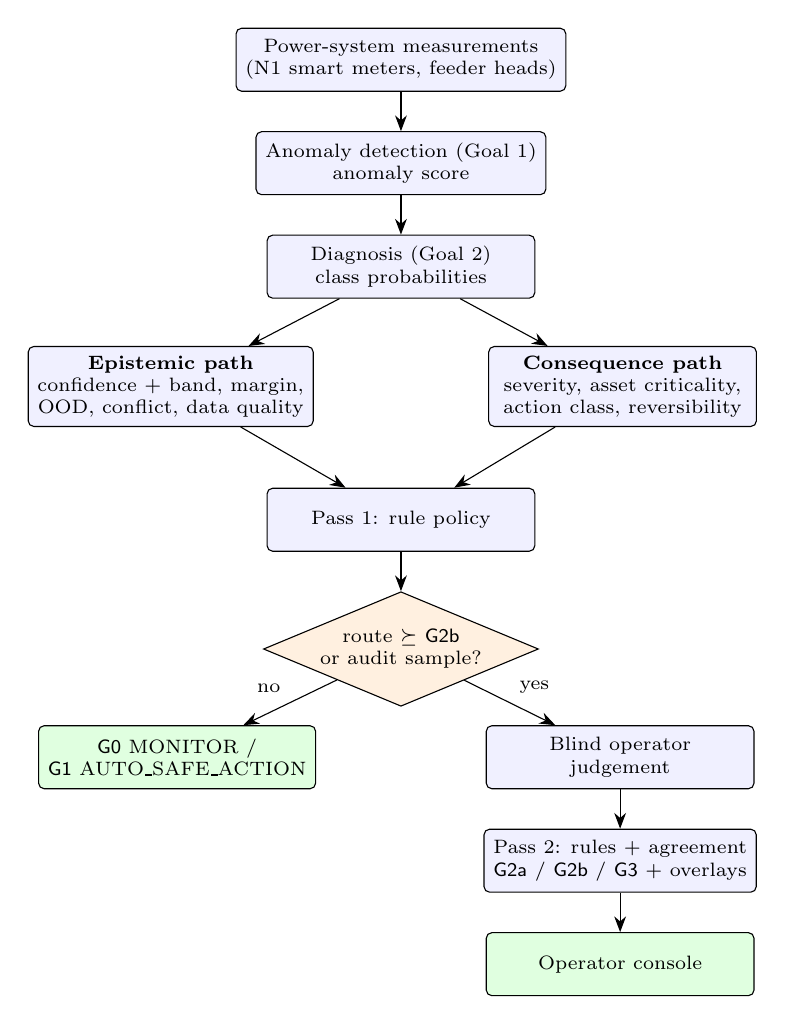
\begin{tikzpicture}[
  b/.style={draw,rounded corners=2pt,align=center,font=\scriptsize,minimum width=34mm,minimum height=8mm,fill=blue!6},
  g/.style={b,fill=green!12}, d/.style={draw,diamond,aspect=2.4,align=center,font=\scriptsize,fill=orange!12,inner sep=1pt},
  >={Stealth[length=2mm]}, node distance=5mm and 8mm]
\node[b] (m) {Power-system measurements\\ (N1 smart meters, feeder heads)};
\node[b,below=of m] (det) {Anomaly detection (Goal 1)\\ anomaly score};
\node[b,below=of det] (dia) {Diagnosis (Goal 2)\\ class probabilities};
\node[b,below left=6mm and -6mm of dia] (ep) {\textbf{Epistemic path}\\ confidence + band, margin,\\ OOD, conflict, data quality};
\node[b,below right=6mm and -6mm of dia] (cp) {\textbf{Consequence path}\\ severity, asset criticality,\\ action class, reversibility};
\node[b,below=24mm of dia] (p1) {Pass 1: rule policy};
\node[d,below=of p1] (q) {route $\succeq$ \lvl{G2b}\\ or audit sample?};
\node[g,below left=6mm and 2mm of q] (g01) {\lvl{G0} MONITOR /\\ \lvl{G1} AUTO\_SAFE\_ACTION};
\node[b,below right=6mm and 2mm of q] (blind) {Blind operator\\ judgement};
\node[b,below=of blind] (p2) {Pass 2: rules + agreement\\ \lvl{G2a} / \lvl{G2b} / \lvl{G3} + overlays};
\node[g,below=of p2] (con) {Operator console};
\draw[->] (m)--(det); \draw[->] (det)--(dia); \draw[->] (dia)--(ep); \draw[->] (dia)--(cp);
\draw[->] (ep)--(p1); \draw[->] (cp)--(p1); \draw[->] (p1)--(q);
\draw[->] (q)--node[above left,font=\scriptsize]{no}(g01); \draw[->] (q)--node[above right,font=\scriptsize]{yes}(blind);
\draw[->] (blind)--(p2); \draw[->] (p2)--(con);
\end{tikzpicture}
\caption{(a) Runtime decision flow.}
\label{fig:runtime}
\end{figure}

\begin{figure}[H]
\centering
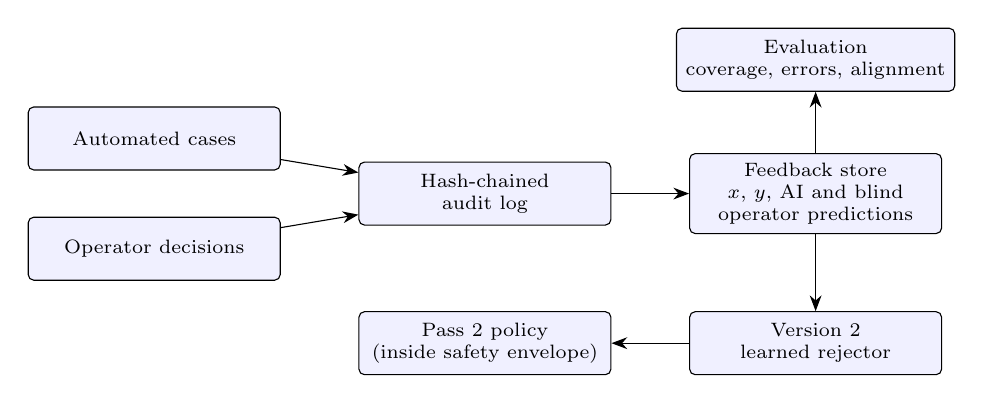
\begin{tikzpicture}[
  b/.style={draw,rounded corners=2pt,align=center,font=\scriptsize,minimum width=32mm,minimum height=8mm,fill=blue!6},
  >={Stealth[length=2mm]}]
\node[b] (auto) at (0,1.2) {Automated cases};
\node[b] (ops) at (0,-0.2) {Operator decisions};
\node[b] (log) at (4.2,0.5) {Hash-chained\\ audit log};
\node[b] (fs) at (8.4,0.5) {Feedback store\\ $x$, $y$, AI and blind\\ operator predictions};
\node[b] (ev) at (8.4,2.2) {Evaluation\\ coverage, errors, alignment};
\node[b] (rej) at (8.4,-1.4) {Version 2\\ learned rejector};
\node[b] (pol) at (4.2,-1.4) {Pass 2 policy\\ (inside safety envelope)};
\draw[->] (auto)--(log); \draw[->] (ops)--(log); \draw[->] (log)--(fs); \draw[->] (fs)--(ev);
\draw[->] (fs)--(rej); \draw[->] (rej)--(pol);
\end{tikzpicture}
\caption{(b) Logging and learning loop.}
\label{fig:loop}
\end{figure}

Three features are deliberate. The epistemic and consequence paths stay separate until the policy is applied,
so confidence cannot dilute risk. The blind judgement sits before the final routing, because the agreement
state is an input to the decision. The learned rejector plugs into the policy rather than replacing it, so the
safety rules keep bounding what it can automate.

\subsubsection{Inputs from the dataset and from Goals 1--2}
The diagnosis classes map one to one onto the labels of the EnergyMind dataset, which provides the ground
truth used in Section~\ref{sec:eval}. Table~\ref{tab:classes} gives the mapping and the event counts of node N1.

\begin{table}[H]
\centering\small
\begin{tabular}{@{}lll r@{}}
\toprule
\textbf{Diagnosis (Goal 2)} & \textbf{Dataset label (\texttt{gt\_label})} & \textbf{Governance handling} & \textbf{N1 events} \\
\midrule
\NORM & \texttt{normal} & \lvl{G0} & -- \\
\GE & \texttt{grid\_event}, \texttt{equipment\_failure} & rules R2, R6 & 33 + 4 \\
\MF & \texttt{sensor\_fault}, \texttt{data\_corruption} & rules R6, R7 & 8 + 25 \\
\SD & \texttt{falsification} & $\ge$ \lvl{G2b} (R6) & 8 \\
\ND & \texttt{comm\_loss} & R0 (input missing) & 20 \\
\bottomrule
\end{tabular}
\caption{Diagnosis classes, dataset labels and event counts in node N1 (98 events in 2025).}
\label{tab:classes}
\end{table}

From Goal~2 the layer receives, per flagged meter-day, the calibrated probability $p(c\mid x)$ of each of the
four classes (multinomial Platt scaling), the confidence band and the rule that fired; from Goal~1, the anomaly
score, the neighbourhood support and the feeder energy-balance alarm. Should only a verdict and its
confidence $c$ be available, the remaining $1-c$ is spread over the other classes in proportion to their
out-of-fold confusion rates, so that the margin and the plausible-hypothesis set below remain defined.

\subsubsection{Five quantities that must not be merged}
\begin{table}[H]
\centering\small
\begin{tabularx}{\textwidth}{@{}>{\raggedright\arraybackslash}p{2.5cm}>{\raggedright\arraybackslash}p{3.6cm}>{\raggedright\arraybackslash}p{3.7cm}L@{}}
\toprule
\textbf{Quantity} & \textbf{Question} & \textbf{Scale} & \textbf{Source} \\
\midrule
Anomaly score $s(x)$ & How unusual are the data? & detector-specific, not a probability & detection layer (Goal 1) \\
AI confidence $p(\hat c\mid x)$ + band & How sure is the diagnosis? & calibrated probability $[0,1]$ & diagnosis model + calibrator (Goal 2) \\
Severity $\sigma$ & How significant is the event technically? & LOW $<$ MEDIUM $<$ HIGH $<$ CRITICAL & severity assessor: scope and duration (Table~\ref{tab:severity}) \\
Asset criticality $\kappa$ & How important is the asset? & LOW $<$ MEDIUM $<$ HIGH $<$ CRITICAL & static asset registry \texttt{configs/assets.yaml} (synthetic overlay, Table~\ref{tab:assets}) \\
Risk $\rho$ & What happens if the governance decision is wrong? & LOW $<$ MEDIUM $<$ HIGH $<$ CRITICAL & derived, Section~\ref{sec:risk} \\
\bottomrule
\end{tabularx}
\caption{Five quantities kept separate.}
\end{table}
A high anomaly score does not imply a confident diagnosis, a confident diagnosis does not imply low risk, and
a severe event may be well understood. Only risk is derived from the others, by an explicit rule.

\paragraph{Asset criticality on the prototype node.} The dataset describes customers (residential classes and
small commercial premises) but contains no hospital, industrial site or other critical asset, and no
criticality field. Criticality is therefore supplied by a small, versioned registry joined on meter and feeder
identifiers (Table~\ref{tab:assets}); the dataset itself is not modified. The critical feeder is an assumption
made so that the critical-asset rules can be exercised.

\begin{table}[H]
\centering\small
\begin{tabularx}{\textwidth}{@{}>{\raggedright\arraybackslash}p{5.2cm}>{\raggedright\arraybackslash}p{2.4cm}L@{}}
\toprule
\textbf{Asset} & \textbf{Criticality} & \textbf{In N1} \\
\midrule
Residential meter (\texttt{res\_small}, \texttt{res\_medium}, \texttt{res\_large}) & LOW & 24 meters \\
Small commercial meter & MEDIUM & 6 meters (F1: 2, F2: 3, F3: 1) \\
Feeder-head meter, feeder switching & HIGH & 3 feeders \\
Feeder N1-F3 (assumed to supply a health centre) & CRITICAL & 10 meters \\
\bottomrule
\end{tabularx}
\caption{Synthetic asset-criticality overlay (\texttt{configs/assets.yaml}). Prototype assumption, not STEG data.}
\label{tab:assets}
\end{table}

\subsubsection{Governance levels}
\begin{table}[H]
\centering\small
\footnotesize
\begin{tabularx}{\textwidth}{@{}>{\raggedright\arraybackslash}p{0.8cm}>{\raggedright\arraybackslash}p{3.3cm}>{\raggedright\arraybackslash}p{3.0cm}>{\raggedright\arraybackslash}p{3.0cm}L@{}}
\toprule
\textbf{Level} & \textbf{Route} & \textbf{Who decides} & \textbf{What may run automatically} & \textbf{Typical case} \\
\midrule
\lvl{G0} & MONITOR & AI & nothing & \NORM, confident, familiar \\
\lvl{G1} & AUTO\_SAFE\_ACTION & AI & whitelisted reversible, non-physical actions & confident meter freeze on a residential meter \\
\lvl{G2a} & AI\_RECOMMENDATION & AI proposes, operator acknowledges & \lvl{G1} actions only & probable meter fault, inspection suggested \\
\lvl{G2b} & HUMAN\_REVIEW & operator, after blind judgement & \lvl{G1} actions only & moderate uncertainty, disagreement, OOD, suspicious data, high risk \\
\lvl{G3} & HUMAN\_APPROVAL\_REQUIRED & named operator with written justification (two people if risk is CRITICAL) & \lvl{G1} actions only; locked actions never run on timeout & breaker or switching operation, disconnection, control-setting change, fraud declaration, critical asset \\
\bottomrule
\end{tabularx}
\caption{Governance levels.}
\end{table}
REQUEST\_MORE\_DATA and SECOND\_REVIEW are procedures that overlay \lvl{G2a}--\lvl{G3}, not levels. In
learning-to-defer terms, \lvl{G0}--\lvl{G1} are ``AI handles'' and \lvl{G2a}--\lvl{G3} are ``defer''.

\subsection{Risk and confidence assessment}
\label{sec:risk}

\subsubsection{Confidence bands}
Let $\hat c=\arg\max_c p(c\mid x)$ be the diagnosis and $p^\star=p(\hat c\mid x)$ its calibrated probability.
With class-specific prototype thresholds $\tau^{\mathrm{low}}_c<\tau^{\mathrm{high}}_c$,
\begin{equation}
\mathrm{band}(x)=\begin{cases}\text{HIGH} & p^\star\ge\tau^{\mathrm{high}}_{\hat c}\\ \text{LOW} & p^\star<\tau^{\mathrm{low}}_{\hat c}\\ \text{MEDIUM} & \text{otherwise}\end{cases}
\qquad \mathrm{margin}(x)=p_{(1)}-p_{(2)} .
\end{equation}
The band is capped at MEDIUM if the input is not in distribution, data quality is not GOOD, or calibration is
not validated for that class, because calibrated probabilities cannot be trusted at face value in those
situations. Prototype values: $\tau^{\mathrm{high}}=0.90$ ($0.85$ for \GE), $\tau^{\mathrm{low}}=0.60$, minimum
margin $0.30$.

\paragraph{When is calibration ``validated''?} A class counts as validated only when its calibration has been
checked on at least 30 out-of-fold events (event-grouped cross-validation, as in Goal~2). In N1 this holds for
\GE{} (37 events) and \MF{} (33), but not for \SD{} (8 events, one per manipulation type). On the prototype node
every \SD{} band is therefore capped at MEDIUM, and with rule R6 every suspicious-data case is reviewed by a
human.

\subsubsection{Severity from scope and duration}
The dataset has no severity field; the severity assessor derives it from how many meters an event touches and
how long it lasts, which Goals~1--2 report (Table~\ref{tab:severity}).

\begin{table}[H]
\centering\small
\begin{tabularx}{\textwidth}{@{}>{\raggedright\arraybackslash}p{6.3cm}>{\raggedright\arraybackslash}p{2.0cm}L@{}}
\toprule
\textbf{Scope and duration} & \textbf{Severity} & \textbf{N1 examples} \\
\midrule
One meter, less than 6 hours & LOW & stuck meter for a few hours, single-house load \\
One meter for 6 hours or more, or 2--6 meters & MEDIUM & long sensor faults, falsification, cable fault (4--6 meters) \\
A whole feeder (10 meters) & HIGH & feeder outage, sag, swell, demand surge \\
The whole node (30 meters) or the transformer & CRITICAL & node-wide outage, transformer degradation and trip \\
\bottomrule
\end{tabularx}
\caption{Severity derivation used on the prototype node.}
\label{tab:severity}
\end{table}

\subsubsection{Risk derivation}
Risk has two sides: acting when we should not, and not acting when we should. The \emph{wrong-action risk} of a
proposed action $a$ on an asset with criticality $\kappa$ is
\begin{equation}
\rho_{\mathrm{act}}(a)=\begin{cases}\max\bigl(\beta(a)\oplus\mathbb 1_{\mathrm{irrev}}(a),\ \kappa\bigr) & \text{if $a$ is physical or customer-affecting}\\
\beta(a)\oplus\mathbb 1_{\mathrm{irrev}}(a) & \text{otherwise}\end{cases}
\end{equation}
where $\beta(a)$ is the base risk of the action class (LOW for informational and data handling, MEDIUM for
operational, HIGH for physical, customer-affecting and accusatory actions) and $\oplus 1$ raises a level by one
step.

The \emph{missed-event risk} uses the severity of the most severe plausible hypothesis, so a confident \MF{}
diagnosis does not hide a plausible \GE:
\begin{equation}
\sigma^\star(x)=\max_{c:\ p(c\mid x)\ge\rho_{\mathrm{plaus}}}\sigma(c),\qquad \rho_{\mathrm{miss}}=M[\kappa,\sigma^\star],
\end{equation}
with $\rho_{\mathrm{plaus}}=0.05$ (prototype) and the ordinal matrix $M$ of Table~\ref{tab:matrix}. Case risk is
the worst of both: $\rho_{\mathrm{case}}=\max\bigl(\rho_{\mathrm{miss}},\ \max_{a\in A}\rho_{\mathrm{act}}(a)\bigr)$.

\begin{table}[H]
\centering\small
\begin{tabular}{@{}lcccc@{}}
\toprule
\textbf{Criticality $\backslash$ Severity} & \textbf{LOW} & \textbf{MEDIUM} & \textbf{HIGH} & \textbf{CRITICAL} \\
\midrule
LOW & LOW & LOW & MEDIUM & HIGH \\
MEDIUM & LOW & MEDIUM & MEDIUM & HIGH \\
HIGH & MEDIUM & MEDIUM & HIGH & CRITICAL \\
CRITICAL & MEDIUM & HIGH & CRITICAL & CRITICAL \\
\bottomrule
\end{tabular}
\caption{Missed-event risk matrix $M[\kappa,\sigma]$.}
\label{tab:matrix}
\end{table}

\paragraph{Why a maximum and not a weighted sum.} The scales are ordinal, so multiplying or averaging their ranks
has no meaning. More importantly, a low value on one dimension must never compensate for a high value on
another: ``low severity'' must not cancel ``health-centre feeder''. The price is conservatism (more
escalations), which is measured by the false-escalation rate (Section~\ref{sec:eval}) rather than assumed
acceptable.

\subsection{Human--AI escalation policy}
\label{sec:policy}

\subsubsection{Routing as a maximum of rule floors}
Order the routes $\lvl{G0}\prec\lvl{G1}\prec\lvl{G2a}\prec\lvl{G2b}\prec\lvl{G3}$. Each rule $R_k$ maps an
event $e$ to a floor $f_k(e)$, with $f_k(e)=\lvl{G0}$ when the rule does not apply. The route is
$\mathrm{route}(e)=\max_k f_k(e)$.

\begin{table}[H]
\centering\small
\footnotesize
\begin{tabularx}{\textwidth}{@{}>{\raggedright\arraybackslash}p{1.9cm}LL>{\raggedright\arraybackslash}p{1.5cm}@{}}
\toprule
\textbf{Rule} & \textbf{Condition} & \textbf{Floor / effect} & \textbf{Tunable} \\
\midrule
R0 Input validity & missing inputs (\ND), unregistered asset, unapproved model version & $\ge$ \lvl{G2b}; \ND{} of 12 intervals or less: \lvl{G1} (gap filling) & no \\
R1 Hard action & physical, customer-affecting, accusatory or irreversible action & action locked; \lvl{G3} & no \\
R2 Consequence & $\rho_{\mathrm{case}}=$ CRITICAL, or $\kappa=$ CRITICAL with a non-\NORM{} diagnosis & $\ge$ \lvl{G2b}, consequential actions locked, two-person approval if CRITICAL risk & no \\
R2b & $\rho_{\mathrm{case}}=$ HIGH & $\ge$ \lvl{G2b} & no \\
R3 Agreement & strong disagreement & $\ge$ \lvl{G2b} + second review + more data + freeze & no \\
R3b & partial disagreement / weak agreement & $\ge$ \lvl{G2b} & no \\
R4 Familiarity & out of distribution / insufficient data & $\ge$ \lvl{G2b} + more data (+ freeze if OOD) & thresholds \\
R5 Confidence & LOW band or strong evidence conflict & $\ge$ \lvl{G2b} + more data & yes \\
R5b & MEDIUM band, small margin or partial conflict & $\ge$ \lvl{G2a} & yes \\
R6 Diagnosis default & \NORM{} $\to$ \lvl{G0}. \MF{} $\to$ \lvl{G1}, but $\ge$ \lvl{G2a} for a voltage offset or clock shift and $\ge$ \lvl{G2b} if it lasts 24~h or more or affects billing (gain drift, bias). \GE{} $\to$ \lvl{G0} if scheduled or self-clearing (load shedding, sag under 30~min, demand surge, cold-load pickup), \lvl{G2a} otherwise, $\ge$ \lvl{G2b} if severity $\ge$ MEDIUM and the cause is equipment. \SD{} $\to$ \lvl{G2b} & floor & yes \\
R7 Recurrence & too many automatic actions on the same asset in a window & $\ge$ \lvl{G2b} & yes \\
R8 Workload & queue strained or overloaded & priority and deadlines only, never the route & yes \\
R9 Consistency & a locked action exists $\to$ \lvl{G3}; a proposed action exists $\to$ $\ge$ \lvl{G2a} & floor & no \\
\bottomrule
\end{tabularx}
\caption{Routing rules. R6 was revised so that, on the prototype node, the route agrees with the dataset's
reference response wherever there is no stated reason to differ (Section~\ref{sec:refpolicy}).}
\label{tab:rules}
\end{table}

\paragraph{Why R6 was revised.} The first version sent every \MF{} to automatic handling (\lvl{G1}) and every
\GE{} to at least \lvl{G2a}. The dataset's reference policy disagrees in two places, and its reasons hold:
a gain drift or a constant bias bills a customer wrongly for weeks, so it needs a human decision (in N1 these
are 8\,922 readings), while scheduled load shedding, short sags and demand surges are routine and only need to
be logged. Voltage offsets and clock shifts, which do not change billing, need an operator to be notified.

\begin{proposition}[Critical consequence dominates confidence]
Fix the diagnosis label $\hat c\ne\NORM$, the asset and the proposed actions. Then, for every value of the AI
confidence $p^\star$: (a) every hard action (physical, customer-affecting, accusatory or irreversible) is locked
and $\mathrm{route}(e)=\lvl{G3}$; (b) if the asset criticality is CRITICAL, $\mathrm{route}(e)\succeq\lvl{G2b}$ and
every proposed non-whitelisted action is locked, so $\mathrm{route}(e)=\lvl{G3}$ whenever one is proposed.
\end{proposition}
\noindent\textit{Proof.} The hard-action condition of R1 depends only on the action catalogue, and the
criticality branch of R2 depends only on $\kappa$ and the label $\hat c$; neither depends on $p^\star$. R1 locks
hard actions; the R2 criticality branch sets a \lvl{G2b} floor and locks every proposed non-whitelisted action;
R9 then sets \lvl{G3} whenever an action is locked. Because the route is a maximum of floors, a change in
$p^\star$ can lower only the floors that depend on it (R4, R5, and R3 through the band), never these. Hence (a)
and (b) hold for all $p^\star$. $\square$

The confidence does influence the missed-event part of the risk, through the plausible hypotheses in
$\sigma^\star$: a more confident diagnosis can rule out a severe alternative. That is intended. Confidence is
allowed to resolve doubt about what happened, never to change what is at stake if the action is wrong. This is
the formal version of the requirement that a 98\%-confident diagnosis on a critical feeder must not trigger
automatic action. The property is also checked by property-based tests on 400 random events in the prototype
code.

\subsubsection{Two-pass evaluation}
\begin{enumerate}[leftmargin=*,itemsep=1pt]
\item Pass 1 applies all rules except R3. If the route is \lvl{G2b} or above, or the case is drawn for the
audit sample, the operator is asked for a blind judgement.
\item Pass 2 adds R3. Since R3 can only raise floors, $\mathrm{route}_2(e)\succeq\mathrm{route}_1(e)$, so the
blind phase never has to be undone.
\end{enumerate}

\subsubsection{Agreement states}
Let $(d_A,b)$ be the AI's diagnosis and band, and $(d_H,h)$ the operator's blind diagnosis and level, with ranks
LOW $=0$, MEDIUM/MID $=1$, HIGH $=2$. A pair of classes is \emph{critical} if confusing them changes the type of
response; in the prototype, the critical pairs are $\{\GE,\MF\}$, $\{\GE,\SD\}$ and $\{\GE,\NORM\}$.
\begin{equation}
\mathrm{agree}(e)=\begin{cases}
\text{NOT\_ASSESSED} & \text{no blind judgement}\\
\text{AGREEMENT} & d_H=d_A,\ \min(b,h)\ge1\\
\text{WEAK\_AGREEMENT} & d_H=d_A,\ \min(b,h)=0\\
\text{PARTIAL} & d_H\ne d_A,\ p(d_H\mid x)\ge\rho_{\mathrm{partial}}\\
\text{STRONG} & d_H\ne d_A,\ p(d_H\mid x)<\rho_{\mathrm{partial}},\ \Gamma(e)\\
\text{PARTIAL} & \text{otherwise}
\end{cases}
\end{equation}
where $\Gamma(e)\equiv(b=h=2)\lor(\{d_A,d_H\}\text{ is a critical pair}\land b\ge1\land h\ge1)$, and
$\rho_{\mathrm{partial}}=0.20$ (prototype).

\begin{table}[H]
\centering\small
\begin{tabularx}{\textwidth}{@{}>{\raggedright\arraybackslash}p{3.2cm}>{\raggedright\arraybackslash}p{5.2cm}L@{}}
\toprule
\textbf{State} & \textbf{Routing effect} & \textbf{Why} \\
\midrule
AGREEMENT & none, never lowers the route & two concordant judgements may share a blind spot \\
WEAK\_AGREEMENT & $\ge$ \lvl{G2b} + more data & same label, but someone is guessing \\
PARTIAL & $\ge$ \lvl{G2b} & competing hypotheses \\
STRONG & $\ge$ \lvl{G2b} + second review + more data + freeze & one party is confidently wrong; resolve by evidence, not authority \\
\bottomrule
\end{tabularx}
\caption{Agreement states and their effect.}
\end{table}
The use of disagreement as an escalation signal is an EnergyMind design decision. It is motivated
by~\cite{benz}, which shows that both confidences carry information and that people move toward the AI's stated
confidence, so the operator's view is only independent if it is captured first.

\subsubsection{Request-more-data loop}
When neither party is confident, the engine schedules information-gathering actions matched to the competing
hypotheses: neighbour measurements, the feeder-head voltage and electrical-consistency checks (\GE{} vs.\
sensor or data problems), history windows and redundant reads (\MF), and the feeder energy balance and the
meter's event log (\SD). All of these are \lvl{G1} actions. The case is then re-evaluated with the new
evidence. The loop is bounded ($\le2$ rounds in the prototype); when the budget is exhausted, the case goes to
a supervisor with no consequential action taken. New evidence may raise the route but never lowers an
escalated case: only a human closes it.

\subsection{Operator interaction}
The console presents a reviewed case in two phases.

\begin{lstlisting}
PHASE 1 - BLIND ASSESSMENT                PHASE 2 - REVEAL AND DECIDE
+-------------------------------------+   +------------------------------------------+
| Evidence only: trends, neighbours,  |   | Your view (locked)   | AI view           |
| data quality, severity, criticality |   | GENUINE_EVENT  HIGH  | METER_FAULT  HIGH |
| (AI diagnosis hidden)               |   |                      | right in 30 of 33 |
|                                     |   |                      | validation events |
| Your diagnosis: [GENUINE_EVENT]     |   | !! STRONG DISAGREEMENT - actions locked  |
| Your confidence: LOW / MID / HIGH   |   | Why here: R3, R6   Data requested: ...   |
| [Submit, show AI view]              |   | [APPROVE] [OVERRIDE] [MORE DATA] [2ND]   |
+-------------------------------------+   +------------------------------------------+
\end{lstlisting}

\paragraph{Against over-trust (automation bias):} blind-first judgement; confidence shown as a band plus a
validated frequency with its real event count (for example ``right in 30 of 33 validation events, simulated''),
and no frequency at all when calibration is not validated for the class (on N1: \SD) or the input is
unfamiliar; the runner-up hypothesis always shown; neutral, equal-size buttons with no default; written
justification for \lvl{G3} approvals and all overrides; two-person approval for CRITICAL risk; monitoring of
approvals that are implausibly fast or frequent. The frequency in the mock-up is illustrative.

\paragraph{Against under-trust:} most routine events never reach the operator (\lvl{G0}/\lvl{G1}), so review
load stays proportionate; per-event-type track records of both AI and operators; outcome feedback showing
operators where the AI was right and they were not, and vice versa; similar past incidents from the log; an
explicit list of situations the model was not validated for; a consistent layout across all cases.

\paragraph{Why the operator is not asked about everything.} The blind judgement is requested only for escalated
cases (\lvl{G2b}, \lvl{G3}) and for a small random audit sample of automatically handled cases (5\% in the
prototype). Escalated cases need a person anyway, so the extra step costs seconds. The audit sample is what makes
errors in the automated region observable at all.

\subsection{Auditability and feedback}
Every decision and human action is appended to the hash-chained decision log shared with Goal~2. Record $k$
stores $\mathrm{hash}_k=\mathrm{SHA256}(\mathrm{record}_k\,\|\,\mathrm{hash}_{k-1})$, so any later edit or
deletion breaks the chain. Goal~2 writes the \texttt{detected}, \texttt{concluded}, \texttt{why} and
\texttt{explanation} blocks; this layer appends a \texttt{governance} block: the assessed consequence (severity,
criticality, per-action risk and gate), the operator's blind and post-reveal judgements, the agreement state,
the route and every rule that fired, data requests, the final decision with its justification, and the policy
and threshold versions. The ground truth and its source are added when available (on the prototype, the dataset
labels). The schema is \texttt{docs/decision\_log\_schema.json} in the project repository.

From the log, the feedback store builds one training record per case with verified outcome,
$(x_i,y_i,\hat y^{\mathrm{AI}}_i,p^\star_i,m_i,h_i,m^{+\mathrm{AI}}_i)$, with correctness indicators
$a_i=\mathbb 1[\hat y^{\mathrm{AI}}_i=y_i]$ and $o_i=\mathbb 1[m_i=y_i]$. Three rules keep these data valid:
\begin{enumerate}[leftmargin=*,itemsep=1pt]
\item The operator's final decision is not ground truth; $y$ comes from simulation labels, field inspection or
later confirmation.
\item The expert label $m$ used for learning is the blind judgement. The post-reveal judgement $m^{+\mathrm{AI}}$
is influenced by the AI, as~\cite{benz} shows, and would teach a rejector to defer to an echo of itself.
\item Automatically handled cases are labelled through the audit sample, so the classifier's error in the region
where it acts alone can be estimated.
\end{enumerate}

\subsubsection{Operator calibration phase}
Before learned deferral can be trained, EnergyMind needs operator decisions with known outcomes. A dedicated
calibration phase collects them efficiently: the console replays labelled events of the dataset, and operators
give a blind diagnosis and confidence with no AI output shown, then see the correct answer (which also serves as
training). This produces, for each operator $o$ and event class $c$, an accuracy estimate
\begin{equation}
\hat a_o(c)=\frac{1}{n_{o,c}}\sum_{i:\ \mathrm{op}(i)=o,\ y_i=c}\mathbb 1[m_i=y_i],
\end{equation}
reported with a confidence interval (e.g.\ Wilson) because $n_{o,c}$ will be small for rare events; node N1 has
only 8 suspicious-data events in a year. A known operator weakness does not by itself justify handing those
cases to the AI. That follows only if the AI is more accurate on the same cases ($\hat a_{\mathrm{AI}}(c)>\hat a_o(c)$
with non-overlapping intervals) and the safety rules R0--R3 allow automation. Where both are weak, the answer
is more data or better sensors, not automation.

\subsection{Future learning-to-defer extension (Version 2)}
\label{sec:v2}
Version~1 is rule-based because EnergyMind has no historical STEG operator decisions. Version~2 replaces only
the tunable rules (R5--R6) with a learned rejector following~\cite{mozannar}. The immutable rules R0--R3 remain
above it as a safety envelope:
\begin{equation}
\begin{gathered}
\mathrm{route}_{V2}(e)=\max\bigl(\mathcal E(e),\ \phi(r_\theta(x))\bigr),\qquad
\mathcal E(e)=\max_{k\in\{R0,R1,R2,R3,R9\}}f_k(e)\ \text{(safety envelope)},\\
\phi(r)=\begin{cases}\lvl{G1} & r=0\ (\text{AI\_HANDLE})\\ \lvl{G2b} & r=1\ (\text{DEFER\_TO\_OPERATOR})\end{cases}\quad\text{(learned rejector $r_\theta$)}
\end{gathered}
\end{equation}
Because of the maximum, the learned rejector can only move cases between automatic handling and review inside
the region the rules already permit to automate. It can never automate a hard action or a critical case.

\begin{figure}[H]
\centering
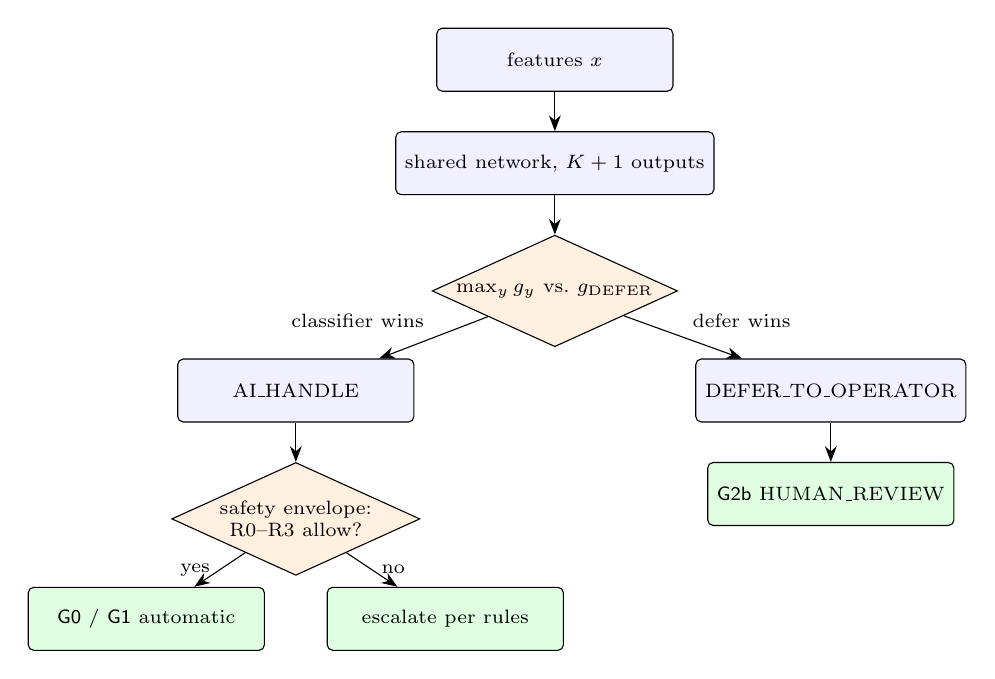
\begin{tikzpicture}[
  b/.style={draw,rounded corners=2pt,align=center,font=\scriptsize,minimum width=30mm,minimum height=8mm,fill=blue!6},
  g/.style={b,fill=green!12}, d/.style={draw,diamond,aspect=2.2,align=center,font=\scriptsize,fill=orange!12,inner sep=1pt},
  >={Stealth[length=2mm]}, node distance=5mm and 10mm]
\node[b] (x) {features $x$};
\node[b,below=of x] (net) {shared network, $K+1$ outputs};
\node[d,below=of net] (cmp) {$\max_y g_y$ vs.\ $g_{\mathrm{DEFER}}$};
\node[b,below left=of cmp] (ah) {AI\_HANDLE};
\node[b,below right=of cmp] (df) {DEFER\_TO\_OPERATOR};
\node[d,below=of ah] (env) {safety envelope:\\ R0--R3 allow?};
\node[g,below left=5mm and -4mm of env] (auto) {\lvl{G0} / \lvl{G1} automatic};
\node[g,below right=5mm and -4mm of env] (esc) {escalate per rules};
\node[g,below=of df] (rev) {\lvl{G2b} HUMAN\_REVIEW};
\draw[->] (x)--(net); \draw[->] (net)--(cmp);
\draw[->] (cmp)--node[above left,font=\scriptsize]{classifier wins}(ah);
\draw[->] (cmp)--node[above right,font=\scriptsize]{defer wins}(df);
\draw[->] (ah)--(env); \draw[->] (df)--(rev);
\draw[->] (env)--node[left,font=\scriptsize]{yes}(auto); \draw[->] (env)--node[right,font=\scriptsize]{no}(esc);
\end{tikzpicture}
\caption{Version 2: the learned rejector inside the rule-based safety envelope.}
\end{figure}

\paragraph{Risk-weighted costs (EnergyMind adaptation).} \cite{mozannar} permits general costs; EnergyMind
uses $\ell(x,y,\hat y)=C[y,\hat y]$ and $\ell_{\exp}(x,y,m)=C[y,m]+c(x)$, where $C$ penalises dangerous
confusions more (e.g.\ predicting \MF{} when the truth is \GE), and $c(x)$ represents operator time, growing with
queue load and urgency. The matrix values are project choices, not literature.

\paragraph{Staged roadmap.}
\begin{enumerate}[leftmargin=*,itemsep=1pt]
\item \textbf{V2-sim} (possible now): train on the dataset's labelled events with synthetic operators of varying
expertise, as~\cite{mozannar} did. This validates the pipeline; it says nothing about real operators.
\item \textbf{V2a}: a confidence-score rejector, estimating $P(M=Y\mid x)$ from calibration-phase and audit data
and deferring when it exceeds $p^\star$ (the empirical version of $r^B$).
\item \textbf{V2b}: joint training of classifier and rejector with $L_{CE}$, once data suffice.
\item \textbf{Shadow mode} before any switch: the learned rejector runs beside V1, decisions are logged but not
used, and it is promoted only if it matches or improves V1 on system error and missed escalations at equal or
lower review load.
\end{enumerate}

\paragraph{Data requirements.} Tuples $(x,y,m)$ with blind $m$; coverage of all four classes and main asset types;
enough operator errors per class (the bound in~\cite{mozannar} depends on the expert error rate); labels in the
automated region; a stable operator population. Neither paper gives a minimum sample size for this domain, and
none is claimed here; on N1 the rare classes alone (8 suspicious-data events) show that one node-year is not
enough.

\subsection{Evaluation strategy}
\label{sec:eval}
The governance layer is evaluated as a human--AI system on the labelled event stream of node N1 (98 events in
2025, plus the clean meter-days), with synthetic operator profiles and, where possible, a small user study.
Let $D$ be the set of deferred cases (\lvl{G2a}--\lvl{G3}) and $A$ the automated cases (\lvl{G0}--\lvl{G1}),
$N=|A|+|D|$. All AI outputs are taken out-of-fold from Goal~2's event-grouped cross-validation, so no event
is routed by a model that was fitted on it.

\begin{table}[H]
\centering\small
\begin{tabularx}{\textwidth}{@{}>{\raggedright\arraybackslash}p{4.0cm}L@{}}
\toprule
\textbf{Metric} & \textbf{Definition} \\
\midrule
Coverage & $|A|/N$ \\
Review rate & cases at \lvl{G2b} or \lvl{G3} $/\,N$ \\
Approval rate & approved \lvl{G3} actions / \lvl{G3} actions \\
Override rate & overrides / reviewed cases \\
Strong-disagreement rate & STRONG / cases with blind judgement \\
False-escalation rate & deferred cases where the AI was right and true risk was below the review level $/\,|D|$ \\
Missed-escalation rate & automated cases where the AI was wrong or true risk required review $/\,|A|$ \\
Unsafe automatic-action rate & inappropriate automatic actions / automatic actions; policy violations must be exactly 0 \\
Agreement with the reference policy & route versus the dataset's \texttt{gt\_expected\_response} (Section~\ref{sec:refpolicy}) \\
AI accuracy on non-deferred & $\frac1{|A|}\sum_{i\in A}a_i$ \\
Operator accuracy on deferred & $\frac1{|D|}\sum_{i\in D}o_i$ (blind) and final-decision accuracy \\
System accuracy & $\frac1N\bigl(\sum_{i\in A}a_i+\sum_{i\in D}\mathbb 1[\mathrm{final}_i=y_i]\bigr)$ \\
Cost-weighted system loss & $\frac1N\sum_i(\ell_i+c_i\mathbb 1[i\in D])$ with $\ell$ from the cost matrix $C$ \\
Reliance & over-reliance: accepted when AI wrong; under-reliance: overridden when AI right; switch rate $m\ne m^{+\mathrm{AI}}$ \\
Response time, workload & median and 90th-percentile decision time per level; cases per operator-hour \\
\bottomrule
\end{tabularx}
\caption{Evaluation metrics of the governance layer.}
\end{table}

\subsubsection{Agreement with the dataset's reference policy}
\label{sec:refpolicy}
Each labelled reading of the dataset carries a suggested response, \texttt{gt\_expected\_response}, presented by
the dataset authors as a starting point for testing escalation logic, not as a standard. It maps onto the
governance levels as in Table~\ref{tab:refmap}. For every event we compare the route with the reference: a
route \emph{below} the reference counts as a missed escalation, a route \emph{above} it as a false escalation,
and the confusion matrix route $\times$ reference is reported. Differences that follow from the asset overlay
(for example a sag on the critical feeder N1-F3, which R2 sends to review while the reference says
\texttt{auto\_log}) are expected and listed separately.

\begin{table}[H]
\centering\small
\begin{tabularx}{\textwidth}{@{}>{\raggedright\arraybackslash}p{3.2cm}>{\raggedright\arraybackslash}p{2.6cm}L@{}}
\toprule
\textbf{Reference response} & \textbf{Nearest route} & \textbf{N1 readings (labels)} \\
\midrule
\texttt{auto\_log} & \lvl{G0} & 1\,100 grid events (load shedding, sag, surge, cold-load pickup), 50 equipment \\
\texttt{auto\_correct} & \lvl{G1} & 112 corruption, 151 stuck meter, 78 short communication losses \\
\texttt{notify\_operator} & \lvl{G2a} & 500 grid events (outage, swell), 3\,711 sensor (voltage offset, clock shift), 351 long communication losses \\
\texttt{human\_decision} & $\ge$ \lvl{G2b} & 14\,175 falsification, 8\,922 sensor (gain drift, bias), 3\,244 equipment failure \\
\bottomrule
\end{tabularx}
\caption{Reference responses of the dataset and their nearest governance level.}
\label{tab:refmap}
\end{table}

\paragraph{Coverage vs.\ performance experiment (after~\cite{mozannar}).} Sort cases by a deferral score $q(x)$
(V1: $q=\tau_{\hat c}-p^\star$; V2-sim: $g_\perp-\max_y g_y$), sweep a threshold to obtain coverage from 0 up to
the coverage ceiling (the share of cases not forced to review by R0--R3), and plot system accuracy, AI accuracy
on non-deferred cases, cost-weighted loss and missed-escalation rate against coverage, one curve per synthetic
operator profile, with the V1 policy as a marked point and operator capacity as a workload line. Hypotheses, not
results: AI accuracy on non-deferred cases falls as coverage rises; system accuracy peaks at intermediate
coverage when operator and AI strengths differ; a V1 point far below the curve means thresholds are misplaced.

\paragraph{Alignment audit (after~\cite{benz}).} One class at a time, with outcome $\mathbb 1[y=c]$, AI confidence
$p(c\mid x)$ in 8 bins and operator level in \{LOW, MID, HIGH\}, estimate the positive rate per cell (cells with
at least 30 samples) and count alignment violations: pairs of cells with higher AI and operator confidence but a
lower positive rate. Summaries:
\begin{align}
\mathrm{EAE}&=\frac1{N_{\mathrm{pairs}}}\sum_{h\le h',\,b\le b'}\bigl[P(Y=1\mid h,b)-P(Y=1\mid h',b')\bigr]_+,\\
\mathrm{MAE}&=\max_{h\le h',\,b\le b'}\bigl[P(Y=1\mid h,b)-P(Y=1\mid h',b')\bigr]_+ .
\end{align}
Also plot $h_{+\mathrm{AI}}-h$ against AI confidence to check whether operators move toward the AI. Many violations
would make multicalibration per operator level a priority for V2. Mapping operator confidence to the one-vs-rest
proposition (their level if they chose $c$, LOW otherwise) is an EnergyMind approximation. On N1 the 30-sample
rule can be met only for \GE{} and \MF; the audit of \SD{} waits for more data.

\paragraph{Testing the out-of-distribution rule (R4).} All three nodes of the dataset come from one generator,
so truly unfamiliar inputs are rare. R4 is exercised on N1's hard-negative periods (Ramadan, August vacations,
heat waves) and on the clock shift of February, which the detectors of Goal~1 do not recognise; in Phase~2, by
running the N1 models on nodes N2 and N3.

\paragraph{Complementarity matrix.} Per event class, asset type, severity and operator profile:
\begin{table}[H]
\centering\small
\begin{tabularx}{\textwidth}{@{}>{\raggedright\arraybackslash}p{2.6cm}LL@{}}
\toprule
 & \textbf{Operator correct ($o=1$)} & \textbf{Operator wrong ($o=0$)} \\
\midrule
\textbf{AI correct ($a=1$)} & both reliable: review adds little; automation candidate if rules allow & AI better: deferral wastes effort; automation candidate if rules allow \\
\textbf{AI wrong ($a=0$)} & operator better (often side information): must stay deferred; what a rejector must learn & neither reliable: more data or sensors; never automate \\
\bottomrule
\end{tabularx}
\caption{Complementarity matrix.}
\end{table}
The ``operator better'' cell contains the positive examples for learned deferral; the ``neither'' cell is a
data-collection target, not a routing problem. This is the empirical counterpart of the complementarity argument
in~\cite{mozannar}.

\subsection{Prototype implementation}
The Version~1 engine is implemented in Python (Pydantic models, YAML policy configuration, hash-chained JSONL
audit log) in \texttt{governance/prototype/}, to be merged into \texttt{src/energymind/govern/} of the project
repository, which already holds the reference-policy check and the asset overlay. The six reference scenarios
run end to end as automated tests, and five safety invariants are verified with property-based tests on 400
random events each. The scenarios are built on real events of node N1 with the asset overlay applied; the AI
output and the operator's answer are scripted test inputs, chosen to exercise each part of the policy.

\begin{table}[H]
\centering\footnotesize
\begin{tabularx}{\textwidth}{@{}>{\raggedright\arraybackslash}p{2.7cm}>{\raggedright\arraybackslash}p{2.7cm}>{\raggedright\arraybackslash}p{2.6cm}L>{\raggedright\arraybackslash}p{1.6cm}@{}}
\toprule
\textbf{Scenario (N1 event)} & \textbf{AI output (scripted)} & \textbf{Key inputs} & \textbf{Outcome} & \textbf{Dataset reference} \\
\midrule
S1 Residential meter freeze (stuck meter, N1-F1, 12--14 Feb) & \MF{} 0.95 (HIGH) & criticality LOW, severity MEDIUM (48~h) & AUTO\_SAFE\_ACTION: quarantine data, re-read, ticket; R6 raises to review if the freeze outlasts 24~h & \texttt{auto\_correct} \\
\addlinespace
S2 Critical-feeder voltage sag (N1-F3, 27 Jun 18:00) & \GE{} 0.98 (HIGH) & criticality CRITICAL (overlay), severity HIGH; transfer to backup feeder proposed & HUMAN\_APPROVAL\_REQUIRED, two-person; sampling and alert run automatically & \texttt{auto\_log} (differs by design: overlay) \\
\addlinespace
S3 Slow gain drift on a customer meter (N1-F2, from 19 Apr) & \MF{} 0.92 (HIGH); operator agrees, HIGH & criticality LOW, billing affected, lasts weeks & HUMAN\_REVIEW (R6 billing rule); agreement does not lower it; quick approval & \texttt{human\_decision} \\
\addlinespace
S4 Demand surge on the most commercial feeder (N1-F2, 23 Jun 18:00) & \MF{} 0.93 (HIGH); operator \GE, HIGH & plausible \GE{} of high severity (10 meters) & STRONG\_DISAGREEMENT: second review, more data, freeze; neighbour evidence confirms the operator & \texttt{auto\_log} \\
\addlinespace
S5 Unfamiliar pattern (clock shift, N1-F1, 23 Feb) & \SD{} 0.46 (LOW), OOD & operator \GE, LOW & HUMAN\_REVIEW, two data rounds, supervisor escalation, no consequential action & \texttt{notify\_operator} \\
\addlinespace
S6 Suspected meter fraud (partial bypass, N1-F2, 4 Feb) & \SD{} 0.94, band capped at MEDIUM; operator agrees & fraud flag and disconnection proposed & HUMAN\_APPROVAL\_REQUIRED, two-person; operator overrides and orders an inspection & \texttt{human\_decision} \\
\bottomrule
\end{tabularx}
\caption{Reference scenarios on node N1. The previous versions of S2 (hospital feeder), S3 (feeder-head meter
drift) and S4 (industrial load) had no counterpart in the dataset: N1 has no hospital or industrial site, and its
feeder-head meters are accurate by construction.}
\end{table}
S2 and S6 illustrate the central claim of the design: high AI confidence, even combined with human agreement,
does not authorise a consequential or accusatory action. S1 and S3 show the revised R6: the same diagnosis
(\MF) is handled automatically for a short freeze and reviewed when it affects a customer's bill for weeks.

\subsection{Research traceability}
A = stated in the paper; B = EnergyMind engineering decision; C = future extension.
\begin{table}[H]
\centering\footnotesize
\begin{tabularx}{\textwidth}{@{}>{\raggedright\arraybackslash}p{3.6cm}>{\raggedright\arraybackslash}p{1.0cm}LL>{\raggedright\arraybackslash}p{1.0cm}@{}}
\toprule
\textbf{Design decision} & \textbf{Source} & \textbf{What the paper actually says} & \textbf{EnergyMind adaptation} & \textbf{Cat.} \\
\midrule
Explicit defer outcome & \cite{mozannar} & predictor outputs a label or $\perp$ & \lvl{G2a}--\lvl{G3} are deferral & A \\
Optimise the combined system & \cite{mozannar} & system loss over classifier and expert & system accuracy, cost-weighted loss & A \\
Coverage and coverage sweep & \cite{mozannar} & coverage = fraction non-deferred; performance vs.\ coverage & sweep up to a safety ceiling & A/B \\
Defer when the expert is more likely right & \cite{mozannar} & Bayes rejector, Proposition~2 & V1 approximates with bands; V2a estimates it & A/B \\
Classifier + rejector, $L_{CE}$ & \cite{mozannar} & joint training with a consistent surrogate & V2b & C \\
$(x,y,m)$ data requirement & \cite{mozannar} & training samples of expert decisions & audit log and calibration phase & A/B \\
Synthetic experts & \cite{mozannar} & used in experiments & synthetic operator profiles, labelled as simulation & A/B \\
Calibration alone insufficient & \cite{benz} & Theorem~3 & operator confidence considered jointly & A \\
Operator confidence before AI advice & \cite{benz} & $H$ formed before observing $B$; data record $h$ and $h_{+\mathrm{AI}}$ & blind-first console & A/B \\
Three operator confidence levels & \cite{benz} & few discrete levels; experiments use three & LOW / MID / HIGH & A \\
People move toward higher AI confidence & \cite{benz} & observed in all four tasks (observational data) & motivates blind-first and band display & A/B \\
Alignment metrics & \cite{benz} & violations, EAE, MAE & one-vs-rest audit & A/B \\
Multicalibration per operator level & \cite{benz} & Theorem~8 & when data allow & C \\
Disagreement states and their effects & neither & not stated & Section~\ref{sec:policy} & B \\
Governance levels, risk, criticality, action classes, thresholds & neither & not stated & Sections~3.3--3.5 & B \\
Asset overlay, severity from scope, reference-policy check & neither & not stated & Sections~3.3, 3.4, 3.9 & B \\
Monotone escalation, safety envelope over learned deferral & neither & \cite{mozannar}'s rejector is unconstrained & Sections~\ref{sec:policy}, \ref{sec:v2} & B \\
Calibration phase, audit sample & neither & not stated & Sections~3.6--3.7 & B \\
\bottomrule
\end{tabularx}
\caption{Research traceability.}
\end{table}

\subsection{Limitations}
\begin{enumerate}[leftmargin=*,itemsep=1pt]
\item \textbf{No real operator data.} Thresholds, the risk matrix and agreement rules are engineering choices for
a simulation and have not been validated with STEG operators.
\item \textbf{Synthetic criticality.} The dataset has no critical assets; the critical feeder, the severity rule
and the scenario AI outputs are assumptions made to exercise the policy.
\item \textbf{Few rare events.} N1 has 8 suspicious-data events in a year, one per manipulation type, so their
calibration cannot be validated and per-type governance results are case studies.
\item \textbf{Conservative by design.} Max-based risk and monotone escalation will over-escalate; this must be
measured, not assumed acceptable.
\item \textbf{Gaps in~\cite{benz}.} Binary theory, lay participants, non-safety tasks, observational data; the
multi-class adaptation is ours.
\item \textbf{Gaps in~\cite{mozannar}.} Single expert distribution, stationarity, no safety constraints, and the
need for $(x,y,m)$ data that do not yet exist.
\item \textbf{Ground truth} for real events may be delayed, ambiguous or never obtained, which biases accuracy
metrics toward easy cases.
\item \textbf{Feedback loops.} The policy decides which cases humans see, so logged data reflect the policy; the
audit sample mitigates this but does not remove it.
\item \textbf{Blind-phase latency} may be unacceptable for urgent cases, where it can be skipped at the cost of
losing the agreement signal.
\item \textbf{Adversarial pressure.} An attacker aware of the policy could try to stay inside the automated
region or flood operators; recurrence limits help but are not a security analysis.
\item \textbf{Simulation and synthetic operators.} All prototype results come from simulated data and simulated
or volunteer operators and must be reported as such.
\end{enumerate}

\begin{thebibliography}{9}
\bibitem{benz} N.~L.~Corvelo Benz and M.~Gomez Rodriguez, ``Human-Aligned Calibration for AI-Assisted Decision
Making,'' arXiv:2306.00074v4, 2024.
\bibitem{mozannar} H.~Mozannar and D.~Sontag, ``Consistent Estimators for Learning to Defer to an Expert,'' in
\emph{Proc.\ 37th International Conference on Machine Learning (ICML)}, PMLR 119, 2020.
\end{thebibliography}
\end{document}
